% "Станет проще"

\documentclass[a4paper,12pt]{article} % тип документа

% report, book

% Рисунки
\usepackage{graphicx}
\usepackage{wrapfig}
\usepackage{hyperref}
\usepackage[rgb]{xcolor}
\pagestyle{plain}
\usepackage{floatflt}
\usepackage{multirow}
\usepackage{lipsum}
\usepackage{amsmath, amstext}
\usepackage{siunitx}
%\usepackage{subcaption}
\usepackage{wrapfig}
\usepackage{mathrsfs}
\usepackage{adjustbox}
\usepackage{enumerate, indentfirst, float}
\usepackage{pgffor}
\usepackage{capt-of, svg}
\usepackage{array}
\usepackage{longtable}
\usepackage{csvsimple}
\usepackage{pdfpages}
\usepackage{subfigure}
\usepackage{sectsty}



%  Русский язык

\usepackage[T2A]{fontenc}			% кодировка
\usepackage[utf8]{inputenc}			% кодировка исходного текста
\usepackage[english,russian]{babel}	% локализация и переносы



% Математика
\usepackage{amsmath,amsfonts,amssymb,amsthm,mathtools} 

\usepackage{wasysym}

%Заговолок
\author{Сафиуллин Роберт	}
\title{Лабораторная работа  4.3.1\\ Изучение дифракции света}





\begin{document} % начало документа

\maketitle


\newpage

\section{Цель работы:}
исследовать явления дифракции Френеля и Фраунгофера на щели
\\
\section{В работе используются:}
оптическая скамья, ртутная лампа, монохроматор, щели с регулироемой шириной, рамка, двойная щель, микроскоп, зрительная труба
 
        


\section{Ход работы}
\textbf{A: Дифракция Френеля} \\


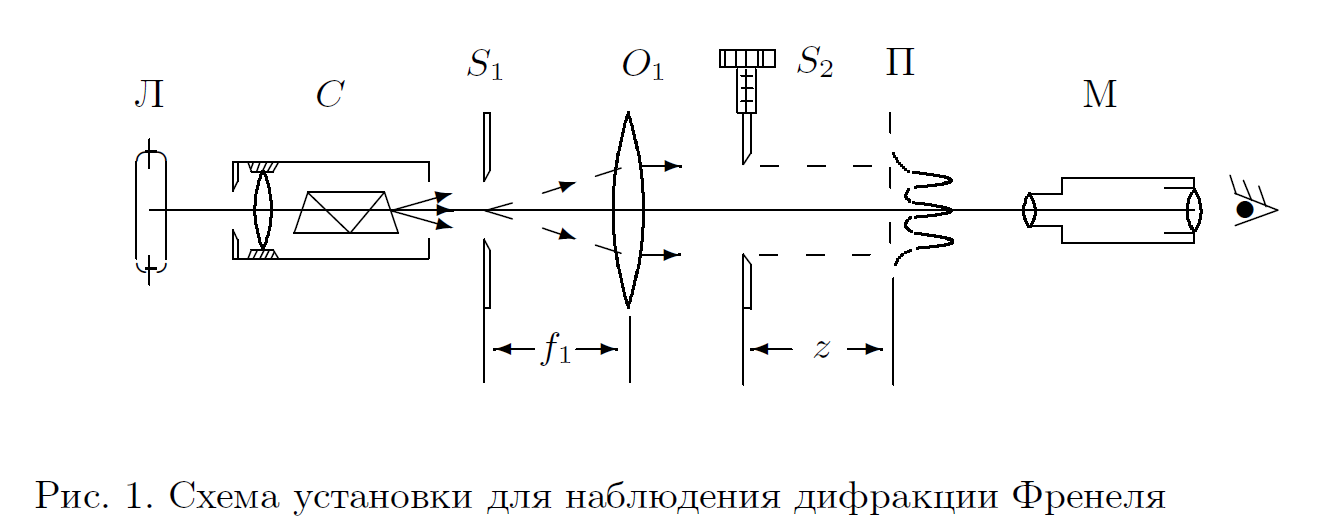
\includegraphics[scale=0.5]{1}

 



 1) Уменьшая расстояние от щели до микроскопа, фиксируем значения расстояний при
появлении новых n темных полос. По формуле $z_m=\sqrt{am\lambda}$, определим ширину m-ой зоны Френеля,
где m – равно числу темных полос плюс 1  (учитывая, что нуль микроскопа - 44.5 см) :
\begin{tabular}{|c|c|c|c|c|c|}
\hline 
n & 1 & 2 & 3 & 4 & 5 \\ 
\hline 
m & 2 & 3 & 4 & 5 & 6 \\ 
\hline 
a, cm & 40.5 & 41.7 & 42.3 & 42.9 & 43.1 \\ 
\hline 
2*$z_m$=b', cm & 418	 & 428.4 & 438.4 & 418& 428.3 \\ 
\hline 
\end{tabular} 
 
Ширина щели b=370 mkm, что отличается от значения b' , полученного по формуле выше. \\

2) Заменим щель препятствием с вертикально расположенной нитью. Наблюдаем светлое пятно Пуассона, находящееся в центре изображения нити.
\\
\textbf{Б: Дифракция Фраунгофера на щели}\\
\begin{center}

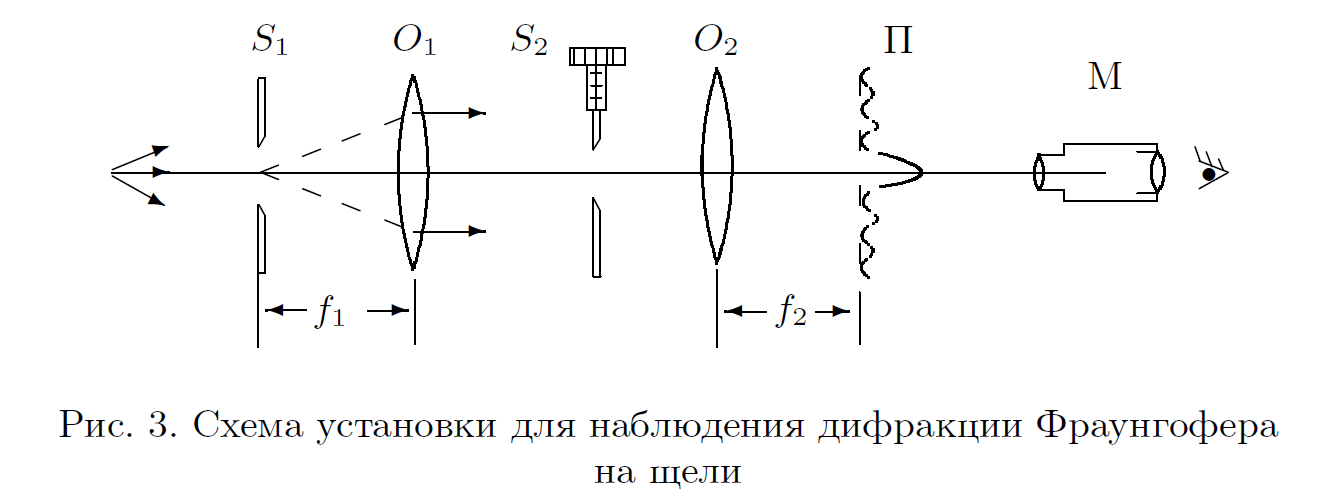
\includegraphics[scale=0.5]{2}
\end{center}
$f_1=12.5 cm  
   , f_2=9 cm $  \\
 3) Измерим с помощью винта поперечного перемещения микроскопа координаты х
нескольких дифракционных минимумов: \\
\begin{tabular}{|c|c|c|c|c|c|c|c|}
\hline 
m & -3 & -2 & -1 & 0 & 1 & 2 & 3 \\ 
\hline 
$x_mm$, del & 0.7	 & 0.79 & 0.91 & 1.05 & 1.19 & 1.28 & 1.4 \\ 
 
\hline 
\end{tabular} 
\\
 4) Пoстроим график зависимости X(m): \\
 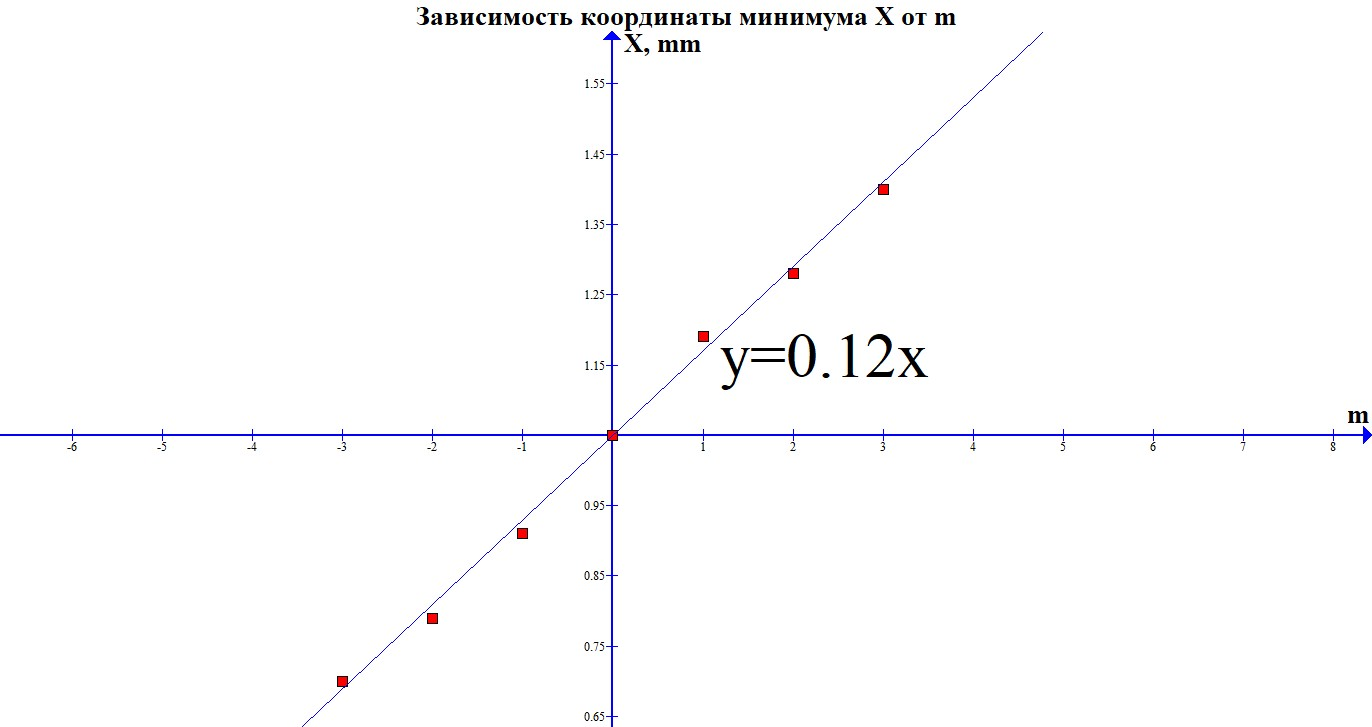
\includegraphics[scale=0.33]{4311}
 \\
 Получили, что среднее расстояние между максимумами $\bigtriangleup X  = 0.12 mm .$ Используя формулу $x_m=\frac{m \lambda f_2}{b}$ вычислим ширину щели: $b = 409.5 mkm,   b_{\text{изм}} = 440 mkm$
 
 
 
 
 
 \textbf{B: Дифракция Фраунгофера на двух щелях} \\
 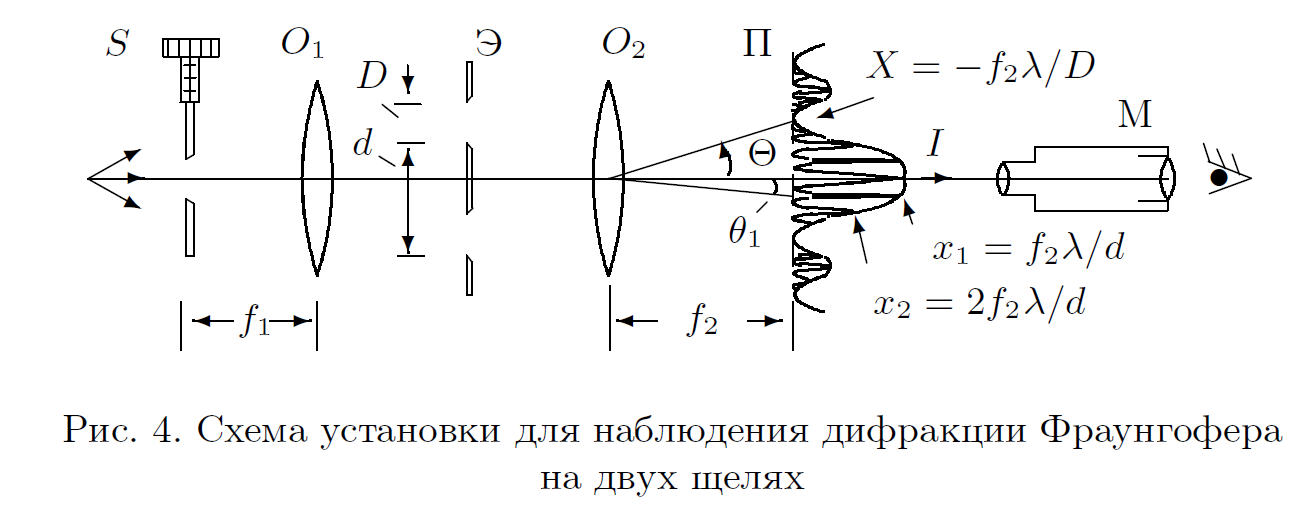
\includegraphics[scale=0.5]{3}
5) Определим координаты самых удаленных друг от друга темных полос внутри
первого максимума, а также координату центра максимума:
$x_1=2.8 mm\\
x_2=3.24 mm\\
$ Между ними находится n = 7 светлых промежутков.\\

$\delta x_{max} = \frac{x_2-x_1}{n} = 62.9 mkm, d= \frac{f_2 \lambda}{\delta x_{max}}=0.78 mm$ \\
Зная ширину щели $b_1$ из следующего пункта, найдем число полос в центральном максимуме: $n'=\frac{2d}{b_1}$ = 8 \\
6) Теперь найдем экспериментально такую ширину щели , при которой исчезают
интерференционные полосы:$_0 $= 191 mkm\\
7) Исследуем влияние просранственной когерентности на видность интерференционной картины. Для этого, расширяя входную щель, подберем значение $b_0=191 mkm$ , при котором наступает первое исчезновение интерференционных полос.
\\


\newpage
\textbf{Г: Влияние дифракции на разрешающую способность оптического инструмента}	\\

\begin{center}

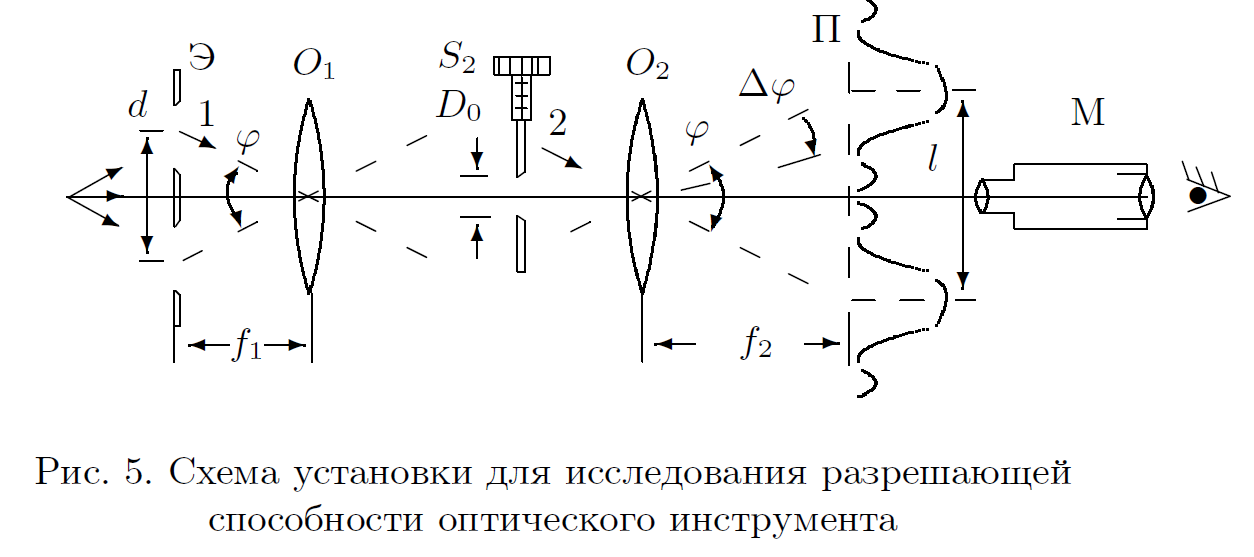
\includegraphics[scale=0.5]{4}

\end{center}


При помощи микроскопа измерим расстояние между щелями: \\
d = 2.45 mm\\
Также получим ширину щелей: \\
$b_1 = 0.6 mm \\
b_2 = 0.32 mm$ \\
Найдем ширину щели при котором пропадают различия между изображениями двух щелей: \\
D= $\frac{f_1 \lambda}{d}$ = 27.3 mkm \\
Теперь экспериментально подберем ширину щели такой, чтобы два изображения
видимые в микроскоп были максимально размыты, но при этом еще видимы:  $ b_0 = 243  mkm$












\end{document} % конец документа
